\section{Example}
\label{sec:example}

\begin{figure}[t]
\centering
\includegraphics[scale=0.8,clip]{figure/dataflow.eps}\vspace*{-3ex}
 \caption
{\label{fig:dataflow}API methods connected by inputs and
outputs}\vspace*{-3ex}
\end{figure}

We next use an example to illustrate challenges involved in
mining API mapping relations. Consider that a programmer needs to translate
a Java code example (shown in Figure~\ref{fig:totranslation}) to C\# using a translation tool.
This code example accepts a \CodeIn{string} input that represents
name of a file or directory and returns a \CodeIn{boolean} value that
describes whether the file or directory exists. To achieve this functionality,
the code example declares a local variable, called \CodeIn{file},
of type \CodeIn{java.io.File} and calls the \CodeIn{exists} method.
We consider \CodeIn{file} as a receiver for the \CodeIn{exists} method.

To translate this code example into C\#, the translation
tool needs to know mapping relations of API classes. For example,
the translation tool needs to know the mapped API class for \CodeIn{java.io.File}
in C\# to translate the variable \CodeIn{file} to C\#. In addition, the translation tool needs
to know the mapped API methods of \CodeIn{exists}. Furthermore,
the translated code should be able to accept the same input
``\CodeIn{test}'' and produce the same output as the Java code example.

To mine mapping relations of APIs, our approach uses existing projects such as
Lucene that have both Java and C\# versions. First, our approach aligns 
classes and methods of the two versions by using 
a matching algorithm based on similarities in the names of classes 
and methods between the two versions. Aligning client code based on names of
classes and methods is based on our observation of how existing
projects such as rasp\footnote{\url{http://sourceforge.net/projects/r-asp/}} are
migrated from one language to another. We observed that while
migrating rasp project from Java to C\#, programmers first rename
source files from Java to C\# and systematically address the
compilation errors by replacing Java APIs with C\# APIs. During this
procedure, names of classes, methods, fields of classes, or local
variables in methods often remain the same between the two versions.
Therefore, we use name similarities for aligning client code of the
two versions. For example, our approach aligns 
\CodeIn{IndexFiles.java} with the \CodeIn{IndexFiles.cs} 
(shown in Figure~\ref{fig:clientcode}) as the names of their classes and methods are similar.

\begin{figure}[t]
\begin{CodeOut}
\begin{alltt}
1  File file = \textbf{new} File("test");
2    \textbf{if}(file.exists())\{...\}
\end{alltt}
\end{CodeOut}\vspace*{-4ex}
\caption{\label{fig:totranslation} A code example for language
translation.}%\vspace*{-1ex}
\end{figure}
\begin{figure}[t]
\begin{CodeOut}\vspace*{-2ex}
\begin{alltt}
                  IndexFiles.java
3 public class IndexFiles \{
4   static final File INDEX_DIR = new File("index");
5   public static void main(String[] args) \{
      ...
6     if (INDEX_DIR.exists()) \{...\}
      ...
7       INDEX_DIR.delete();
    \}
  \}
                  IndexFiles.cs
8 class IndexFiles\{
9   internal static readonly System.IO.FileInfo INDEX_DIR
          = new System.IO.FileInfo("index");
10   public static void  Main(System.String[] args)\{
      ...
11     bool tmpBool;
12     if (System.IO.File.Exists(INDEX_DIR.FullName))
13       tmpBool = true;
14    else
15       tmpBool = System.IO.Directory
                         .Exists(INDEX_DIR.FullName);
      ...
    \}
 \}
\end{alltt}
\end{CodeOut}\vspace*{-4ex}
\caption{\label{fig:clientcode} Two versions (Java and C\#) of
client code.}\vspace*{-4ex}
\end{figure}

Next, our approach mines mapping relations of API classes by comparing entities such as
names of fields in aligned classes, or variable names or constants in aligned methods. 
Figure~\ref{fig:dataflow} shows how our approach maps variables and constants in aligned methods 
of the client code. Our approach uses a text-based similarity measure for comparing these entities
and considers the entities as similar if the measure is greater than a given threshold.
These mapping relations of API classes help translate variables from one language to another. 
For example, our approach identifies the constant value ``\CodeIn{index}'',
in Lines 4 (Java) and 9 (C\#) (Figure~\ref{fig:clientcode}) and
maps the API classes associated with these constants. 
Using this constant value, our approach maps the API
class \CodeIn{java.io.File} of Java to \CodeIn{System.IO.FileInfo} of C\#.  

After mapping API classes between the two languages, our approach maps
API methods. Mapping API methods is challenging as often an API method of one language
can be mapped to multiple API methods of the other language. Furthermore,
mapping relations of API methods should also describe how parameters and return
values are mapped between them. To address these challenges, our approach constructs a
graph, referred as \emph{API transformation graph} (ATG), for
aligned methods of the client code in both languages. These ATGs
precisely capture inputs and outputs of API methods, and help mine
mapping relations of API methods. Figure~\ref{fig:example} shows a mapping
relation between API method \CodeIn{Exist} from one language to another.
Section~\ref{sec:approach:mappingtypes} presents more details on how we mine these mapping relations
of API methods using ATGs.

\begin{figure}[t]
\centering
\includegraphics[scale=0.65,clip]{figure/sample.eps}\vspace*{-3ex}
 \caption
{\label{fig:example}API mapping}\vspace*{-3ex}
\end{figure}

%Based on the mapping relations, a translation tool can migrate the
%preceding code snippet automatically. To learn the mapping
%relations,
%
%%\begin{figure}[t]
%%\centering
%%\includegraphics[scale=0.86,clip]{figure/openfile.eps}\vspace*{-1.5ex}
%% \caption
%%{\label{fig:openfile}Aligned client code}\vspace*{-2ex}
%%\end{figure}
%
%In this section, we illustrate the main steps of our approach to
%mine the API mapping in Java for \CodeIn{System.IO.Directory.
%Exists()} in C\# from the HypoLog
%project\footnote{\url{http://sourceforge.net/projects/twlog/}}.
%
%The first step of our approach is to align classes and methods of
%client code by names. This step finds class pairs and method pairs
%that implement similar functionalities, and each pair may use
%API mapping since it implements a similar functionality. Our
%approach chooses names to align classes and methods because these
%classes and methods are from the same project. In this example, our
%approach aligns the two methods as shown in
%Figure~\ref{fig:openfile} because the two method have similar names
%and their declaring classes also have similar names (see
%Section~\ref{sec:approach:alignclientcode} for details).
%
%The second step of our approach is to mine mapping relations of API
%classes based on the names of corresponding fields, parameters,
%returned types, and local variables. This step also relies on names
%for the same consideration of the first step. For example, our
%approach maps the two parameters with the same name as shown by the
%red arrow of Figure~\ref{fig:openfile}. From the types of the two
%parameters, our approach mines the mapping relation between two API
%classes: \CodeIn{System.String} $\leftrightarrow$
%\CodeIn{java.lang.String} (see
%Section~\ref{sec:approach:mappingtypes} for details).
%
%
%The final step of our approach is to mine mapping relations of API
%methods. Besides the factors listed in
%Section~\ref{sec:introduction}, another factor is that API calls in
%client code are often not carefully aligned. To deal with those
%challenges, our approach first builds an API Transformation Graph
%(ATG) for each method. After that, our approach compares built
%graphs to mine mapping relations of API methods (see
%Section~\ref{sec:approach:mappingtypes} and
%Figure~\ref{fig:approach1} for details). Figure~\ref{fig:example}
%shows the mined mapping relation between
%\CodeIn{System.IO.Directory.Exists()} and its API mapping in
%Java.
